\documentclass{article}
\usepackage[margin=.9in]{geometry}
\usepackage{xcolor}
\usepackage{amsmath, amsthm}
\usepackage{amssymb}
\usepackage{mathrsfs}
\usepackage{tikz}
\usepackage{csquotes}
\usepackage{float}
\newtheorem*{claim}{Claim}
\newtheorem{lemma}{Lemma}
\newtheorem*{poof}{Proof}

\title{Class Portfolio}
\author{Christopher Hunt}
\date{}

\usepackage{graphicx} 
\usepackage{fancyhdr}

\begin{document}
\pagestyle{fancy}
\fancyhf{}
\rfoot{MTH 231}
\lfoot{Christopher Hunt}
\lhead{Class Portfolio}
\rhead{\thepage}

\maketitle

\section*{22. Suppose that a particular real number 
 has the property that $x+\frac{1}{x}$ is an integer. Prove that $x^n+\frac{1}{x^n}$ is an integer for all natural numbers.}

\begin{claim}
     $x^n+\frac{1}{x^n}$ is an integer for all natural numbers.
     \[\forall n \in \mathbb{N}, x^n +\frac{1}{x^n}\text{ \emph{is an integer}}\]
\end{claim}
\begin{poof}
     Let's begin by considering the base case where n = 1.
    \begin{align*}
         x^1+&\frac{1}{x^1}\\         x+&\frac{1}{x}
    \end{align*}
    Since $x+\frac{1}{x}$ is assumed to be an integer we can state that the claim where n=1, is true.
    \\
    
    \noindent Now let us assume for all integers from 0 to k the claim holds true. Since we know that integers have closure under multiplication if we multiplied the integer $x^k+\frac{1}{x^k}$ by $x+\frac{1}{x}$ the product will be an integer. Consider the expansion of this product equals some integer j.
    \begin{align*}
        (x^k+\frac{1}{x^k})(x+\frac{1}{x})=&\,j\\
        x^{k}x+\frac{x^k}{x}+\frac{x}{x^k}+\frac{1}{x^{k}x}=&\,j\\
        x^{k+1}+\frac{1}{x^{k+1}}+x^{k-1}+\frac{1}{x^{k-1}}=&\,j\\
    \end{align*}
    Since we are assuming that the claim holds for all values up to k, it will then hold true for $k-1$. We can replace $x^{k-1}+\frac{1}{x^{k-1}}$ for some integer $m$
    \begin{align*}
        x^{k+1}+\frac{1}{x^{k+1}}+x^{k-1}+\frac{1}{x^{k-1}}=&\,j\\
        x^{k+1}+\frac{1}{x^{k+1}}+m=&\,j
    \end{align*}
    Since we know that both j and m are integers and integers are closed under addition the sum of $x^{k+1}+\frac{1}{x^{k+1}}$ must also be an integer. Therefore by strong induction, the claim is true.
    \\
    \qed\end{poof}
\newpage
\section*{SQ-4. For all sets $A$ and $B$,}
\subsection*{a. Prove that $A$ is a subset of $B$ if and only if $B^c$ is a subset of $A^c$.}
To begin this proof we must start with proving that the cardinality of a subset of a set is less than or equal to the cardinality of the set itself.
\begin{claim}
    $A \subseteq B \rightarrow |A| \leq |B|$
\end{claim}
\begin{lemma}
    To prove this we will use proof by contradiction. Suppose the claim were not the case, then $A \subseteq B \wedge |A| > |B|$. This means that there must be at least one element in $A$ that is not also in $B$, in order for this to be true $A$ could not be a subset of $B$ by the definition of subsets. Therefore the claim is true by contradiction.
\end{lemma}
    
\begin{claim}
    $A \subseteq B \leftrightarrow B^c \subseteq A^c$
\end{claim}
\begin{poof}
    This bidirectional claim can be broken down into two implications:
    \begin{align*}
        1.&\;A\subseteq B \rightarrow B^c\subseteq A^c\\
        2.&\;B^c\subseteq A^c \rightarrow A\subseteq B
    \end{align*}
    Let's assume the antecedant of claim one to be true. That is $A$ is a subset of $B$.
    \begin{figure}[H]
    \centering
        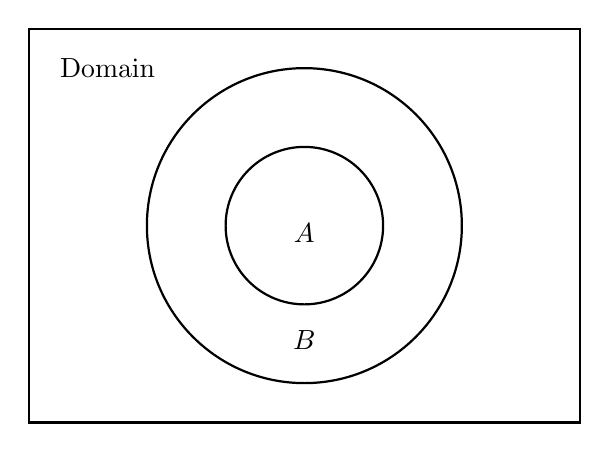
\begin{tikzpicture}[thick]
          % Draw box
          \draw (-3.5cm,-2.5cm) rectangle (3.5cm,2.5cm);
          \node[text=black] at (-2.5cm, 2) {Domain};
          % Draw middle circle (B)
          \draw (0,0) circle (2cm);
          \node[text=black] at (0,-1.45cm) {$B$};
          % Draw inner circle (A)
          \draw (0,0) circle (1cm);
          \node[text=black] at (0,-.10cm) {$A$};
        \end{tikzpicture}
    \end{figure}
    Now consider $B^c$ and $A^c$ which are the areas in the domain which are outside the corresponding sets of $A$ and $B$. Since every element of $A$ is in $B$ we know that $A$ has less than or equal to the same number of elements as $B$ by Lemma 1. Taking their compliment we know that $B^c$ is less than or equal to $A^c$ and since all the elements in $A$ are also in $B$, we know that any element which is not in $B$ must also not be in $A$ which meets the definition of a subset. Therefore the implication is true.

    Now Let's assume the antecedent of the second claim is true. That is every element not in $B$ is also not in $A$.
    \begin{figure}[H]
        \centering
            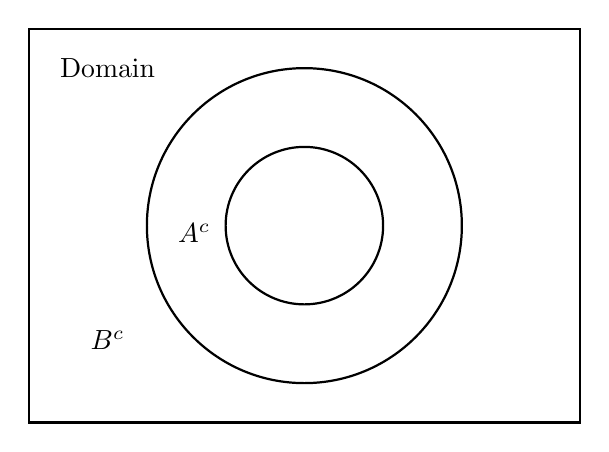
\begin{tikzpicture}[thick]
              % Draw box
              \draw (-3.5cm,-2.5cm) rectangle (3.5cm,2.5cm);
              \node[text=black] at (-2.5cm, 2) {Domain};
              % Draw middle circle (B)
              \draw (0,0) circle (2cm);
              \node[text=black] at (-2.5cm,-1.45cm) {$B^c$};
              % Draw inner circle (A)
              \draw (0,0) circle (1cm);
              \node[text=black] at (-1.4cm,-.10cm) {$A^c$};
            \end{tikzpicture}
        \end{figure}
    Due to this fact every element not in $A^c$ must also not be in $B^c$, that is every element in $A$ is also in $B$. Therefore the second claim holds. Since both claims are true then the original claim is also true. \\
    \qed\end{poof}


\subsection*{b. Prove that if $A$ is a subset of $B$ and $B$ is a subset of $A$, then $A=B$.}
\begin{claim}
    $A \subseteq B \wedge B \subseteq A \rightarrow A = B$
\end{claim}
\begin{poof}
    Assume that $A \subseteq B$ and $B \subseteq A$ are both true. That is, every element of $A$ is an element of $B$ and every element of $B$ is an element of $A$. Consider some arbitrary element $x$ in the set $A$, this element will be in set $B$. Now, consider some other arbitrary element $y$ in set $B$, this element will be in set $A$ as well. Since there are no elements that can be found in $A$ that are not in $B$ and no elements that can be found in $B$ that are not in $A$, therefore $A$ and $B$ contain exactly the same elements. Therefore the claim is true. \\ 
    \qed\end{poof}

\end{document}